\documentclass{article}

%% Useful packages
\usepackage{graphicx} % Required for inserting images
\usepackage{fullpage,enumitem,amsmath,amssymb,url,hyperref}
\usepackage{sectsty}
\usepackage{tgpagella}
\usepackage{tcolorbox}
\usepackage{float}
\usepackage{booktabs}
\usepackage{microtype}
\usepackage{bm}
\usepackage[skip=10pt plus1pt, indent=0pt]{parskip}
\usepackage[edges]{forest} % file structure
\usepackage{cleveref}
\hypersetup{
    colorlinks=true,
    linkcolor=blue,
}

%% Title formatting
\makeatletter
\def\@maketitle{%
  \newpage
  \null
  \begin{center}%
  \let \footnote \thanks
    {\LARGE {\@title}\par}%
    {\@author}%
  \end{center}%
  \par
}
\makeatother

%% Useful math variables
% Random variables
\def\ra{{\textnormal{a}}}
\def\rs{{\textnormal{s}}}

% Random vectors
\def\rva{{\mathbf{a}}}
\def\rvs{{\mathbf{s}}}

% Elements of random vectors
\def\erva{{\textnormal{a}}}
\def\ervs{{\textnormal{s}}}

% Vectors
\def\vzero{{\bm{0}}}
\def\vone{{\bm{1}}}
\def\vmu{{\bm{\mu}}}
\def\vtheta{{\bm{\theta}}}
\def\va{{\bm{a}}}
\def\vs{{\bm{s}}}

\title{CAS4160 Homework 2: Policy Gradients}
\author{
    \textbf{Kyeongwoo Lee} \\
    \textbf{2021147505}
}

\begin{document}

\maketitle

\section{Introduction}

The goal of this assignment is to help you understand \textbf{Policy Gradient Methods}, including variance reduction tricks, such as reward-to-go, neural network baselines, and Generalized Advantage Estimator (GAE). Finally, you will implement Proximal Policy Optimization (PPO), a widely used on-policy RL algorithm that works very well in practice. Here is the link to \href{https://www.overleaf.com/read/xtwbvpnqgxrn#0fb229}{this homework report template in Overleaf}.

\section{Review}

\subsection{Policy Gradient}
Recall that the reinforcement learning objective is to learn $\theta^{*}$ that maximizes the objective function:
\begin{equation}
    J(\theta)=\mathbb{E}_{\tau \sim \pi_{\theta}(\tau)}[r(\tau)],
\end{equation}
where each rollout $\tau$ is of length $T$, as follows:
\begin{equation*}
    \pi_\theta(\tau) = p\left(\rvs_0, \rva_0, \ldots, \rvs_{T-1}, \rva_{T-1}, \rvs_T \right) = p\left(\rvs_0\right) \prod_{t=0}^{T-1} \pi_\theta\left(\rva_t \mid \rvs_t \right) p\left(\rvs_{t+1} \mid \rvs_{t}, \rva_{t}\right),
\end{equation*}
and
\begin{equation*}
    r(\tau)=r\left(\rvs_0, \rva_0, \ldots, \rvs_{T-1}, \rva_{T-1}\right) = \sum_{t=0}^{T-1} r\left(\rvs_t, \rva_t\right).
\end{equation*}
\textbf{Note:} In this assignment, $t$ starts from $0$, not from $1$, which is easier to implement.

The policy gradient approach is to directly take the gradient of this objective:
\begin{align*}
    \nabla_{\theta} J(\theta) & = \nabla_{\theta} \mathbb{E}_{\tau \sim \pi_{\theta}(\tau)}[r(\tau)] & \\
                                & =\nabla_{\theta} \int \pi_{\theta}(\tau) r(\tau) d \tau &  \\
                                & =\int \pi_{\theta}(\tau) \nabla_{\theta} \log \pi_{\theta}(\tau) r(\tau) d \tau & (\because \nabla_\theta \pi_\theta(\tau) = \pi_\theta(\tau) \nabla_\theta \log \pi_\theta(\tau)) \\
                                & =\mathbb{E}_{\tau \sim \pi_{\theta}(\tau)}\left[\nabla_{\theta} \log \pi_{\theta}(\tau) r(\tau)\right]. &
\end{align*}

In practice, the expectation over trajectories $\tau$ can be approximated from a batch of $N$ sampled trajectories:
\begin{align}
    \nabla_{\theta} J(\theta) & \approx \frac{1}{N} \sum_{i=1}^{N} \nabla_{\theta} \log \pi_{\theta}\left(\tau_{i}\right) r\left(\tau_{i}\right) \nonumber \\
                                & =\frac{1}{N} \sum_{i=1}^{N}\left(\sum_{t=0}^{T-1} \nabla_{\theta} \log \pi_{\theta}\left(\rva_{i t} \mid \rvs_{i t}\right)\right)\left(\sum_{t=0}^{T-1} r\left(\rvs_{i t}, \rva_{i t}\right)\right). \label{eq:pg}
\end{align}

Here, we see that the policy $\pi_{\theta}$ is a probability distribution over the action space, conditioned on the state. In the agent-environment loop, the agent samples an action $\rva_{t}$ from $\pi_{\theta}\left(\cdot \mid \rvs_{t}\right)$ and the environment responds with a reward $r\left(\rvs_{t}, \rva_{t}\right)$.

\subsection{Variance Reduction}

\subsubsection{Reward-to-go}

One way to reduce the variance of the policy gradient is to exploit causality: the notion that the policy cannot affect the rewards in the past. This yields the following modified objective, where the sum of rewards here does not include the rewards achieved prior to the time step at which the policy is being queried. This sum of rewards is a sample estimate of the $Q$ function, and is referred to as the ``reward-to-go'':
\begin{equation} \label{eq:pg_rtg}
    \nabla_{\theta} J(\theta) \approx \frac{1}{N} \sum_{i=1}^{N} \sum_{t=0}^{T-1} \nabla_{\theta} \log \pi_{\theta}\left(\rva_{i t} \mid \rvs_{i t}\right)
    \underbrace{\left(
    \sum_{t^{\prime}=t}^{T-1} r\left(\rvs_{i t^{\prime}}, \rva_{i t^{\prime}}\right)
    \right)}_\textrm{reward-to-go}.
\end{equation}

\subsubsection{Discounting}

Multiplying a discount factor $\gamma$ to the rewards can be interpreted as encouraging the agent to focus more on the rewards that are closer in time, and less on the rewards that are further in the future. This can also be thought of as a means for reducing variance as there can be more variance and uncertainty when considering faraway futures.

We can apply the discount on the rewards from full trajectory in \Cref{eq:pg}:
\begin{equation} \label{eq:pg_discount}
    \nabla_{\theta} J(\theta) \approx \frac{1}{N} \sum_{i=1}^{N}\left(\sum_{t=0}^{T-1} \nabla_{\theta} \log \pi_{\theta}\left(\rva_{i t} \mid \rvs_{i t}\right)\right)\left(\sum_{t^{\prime}=0}^{T-1} \gamma^{t^{\prime}-1} r\left(\rvs_{i t^{\prime}}, \rva_{i t^{\prime}}\right)\right).
\end{equation}

We can also apply the discount on the ``reward-to-go'' in \Cref{eq:pg_rtg}:
\begin{equation} \label{eq:pg_rtg_discount}
    \nabla_{\theta} J(\theta) \approx \frac{1}{N} \sum_{i=1}^{N} \sum_{t=0}^{T-1} \nabla_{\theta} \log \pi_{\theta}\left(\rva_{i t} \mid \rvs_{i t}\right)\left(\sum_{t^{\prime}=t}^{T-1} \gamma^{t^{\prime}-t} r\left(\rvs_{i t^{\prime}}, \rva_{i t^{\prime}}\right)\right).
\end{equation}

\subsubsection{Baseline}

Another variance reduction method is to subtract a baseline (that is only conditioned on the current state $\rvs_t$) from the sum of rewards:
\begin{equation}
    \nabla_{\theta} J(\theta)=\mathbb{E}_{\tau \sim \pi_{\theta}(\tau)}\left[\sum_{t=0}^{T-1} \nabla_{\theta} \log \pi_\theta(\rva_t \mid \rvs_t) [r(\tau)-b(\rvs_t)]\right].
\end{equation}
This leaves the policy gradient unbiased because
\begin{align*}
    \mathbb{E}_{\tau \sim \pi_{\theta}(\tau)}[\nabla_{\theta} \log \pi_\theta(\rva_t \mid \rvs_t) b(\rvs_t)]
            &= \mathbb{E}_{\tau \sim \pi_{\theta}(\tau)}[\nabla_{\theta} \log \pi_\theta(\rva_t \mid \rvs_t)] \mathbb{E}_{\tau \sim \pi_{\theta}(\tau)}[b(\rvs_t)] \\
            &= 0 \cdot \mathbb{E}_{\tau \sim \pi_{\theta}(\tau)}[b(\rvs_t)] = 0.
\end{align*}

In this assignment, we will implement a value function $V_{\phi}^{\pi}(\rvs_t)$, which acts as a state-dependent baseline. This value function will be trained to approximate the sum of future rewards starting from a particular state:
\begin{equation}
    V_{\phi}^{\pi}\left(\rvs_{t}\right) \approx \sum_{t^{\prime}=t}^{T-1} \mathbb{E}_{\tau \sim \pi_{\theta}(\tau)}\left[r\left(\rvs_{t^{\prime}}, \rva_{t^{\prime}}\right) \mid \rvs_{t}\right].
\end{equation}
Then, the approximate policy gradient now looks like this:
\begin{equation}
    \nabla_{\theta} J(\theta) \approx \frac{1}{N} \sum_{i=1}^{N} \sum_{t=0}^{T-1} \nabla_{\theta} \log \pi_{\theta}\left(\rva_{i t} \mid \rvs_{i t}\right)\left(
        \underbrace{\left(\sum_{t^{\prime}=t}^{T-1} \gamma^{t^{\prime}-t} r\left(\rvs_{i t^{\prime}}, \rva_{i t^{\prime}}\right)
    \right)}_\textrm{reward-to-go}
    -
    \underbrace{V_{\phi}^{\pi}\left(\rvs_{i t}\right)}_\textrm{baseline}\right).
\end{equation}

\subsubsection{Generalized Advantage Estimator (GAE)}

The quantity $\left(\sum_{t^{\prime}=t}^{T-1} \gamma^{t^{\prime}-t} r\left(\rvs_{t^{\prime}}, \rva_{t^{\prime}}\right)\right)-V_{\phi}^{\pi}\left(\rvs_{t}\right)$ from the previous policy gradient expression (removing the index $i$ for clarity) can be interpreted as an estimate of the advantage function:
\begin{equation}
    A^{\pi}\left(\rvs_{t}, \rva_{t}\right)=Q^{\pi}\left(\rvs_{t}, \rva_{t}\right)-V^{\pi}\left(\rvs_{t}\right),
\end{equation}
where $Q^{\pi}\left(\rvs_{t}, \rva_{t}\right)$ is estimated using Monte Carlo returns and $V^{\pi}\left(\rvs_{t}\right)$ is estimated using the learned value function $V_{\phi}^{\pi}$. We can further reduce variance by also using $V_{\phi}^{\pi}$ in place of the Monte Carlo returns to estimate the advantage function as:
\begin{equation}
    A^{\pi}\left(\rvs_{t}, \rva_{t}\right) \approx \delta_{t}=r\left(\rvs_{t}, \rva_{t}\right)+\gamma V_{\phi}^{\pi}\left(\rvs_{t+1}\right)-V_{\phi}^{\pi}\left(\rvs_{t}\right),
\end{equation}
with the edge case $\delta_{T-1}=r\left(\rvs_{T-1}, \rva_{T-1}\right)-V_{\phi}^{\pi}\left(\rvs_{T-1}\right)$. However, this comes at the cost of introducing bias to our policy gradient estimate, due to modeling errors in $V_{\phi}^{\pi}$. We can instead use a combination of $n$-step Monte Carlo returns and $V_{\phi}^{\pi}$ to estimate the advantage function as:
\begin{equation}
    A_{n}^{\pi}\left(\rvs_{t}, \rva_{t}\right)=\sum_{t^{\prime}=t}^{t+n} \gamma^{t^{\prime}-t} r\left(\rvs_{t^{\prime}}, \rva_{t^{\prime}}\right)+\gamma^{n} V_{\phi}^{\pi}\left(\rvs_{t+n+1}\right)-V_{\phi}^{\pi}\left(\rvs_{t}\right).
\end{equation}

Increasing $n$ incorporates the Monte Carlo returns more heavily in the advantage estimate, which lowers bias and increases variance, while decreasing $n$ does the opposite. Note that $n=T-t-1$ recovers the unbiased but higher variance Monte Carlo advantage estimate used in (13), while $n=0$ recovers the lower variance but higher bias advantage estimate $\delta_{t}$.

We can combine multiple $n$-step advantage estimates as an exponentially weighted average, which is known as the generalized advantage estimator (GAE). Let $\lambda \in[0,1]$. Then, we define:
\begin{equation}
    A_{GAE}^{\pi}\left(\rvs_{t}, \rva_{t}\right)=\frac{1-\lambda^{T-t-1}}{1-\lambda} \sum_{n=1}^{T-t-1} \lambda^{n-1} A_{n}^{\pi}\left(\rvs_{t}, \rva_{t}\right),
\end{equation}
where $\frac{1-\lambda^{T-t-1}}{1-\lambda}$ is a normalizing constant. Note that a higher $\lambda$ emphasizes advantage estimates with higher values of $n$, and a lower $\lambda$ does the opposite. Thus, $\lambda$ serves as a control for the bias-variance tradeoff, where increasing $\lambda$ decreases bias and increases variance. In the infinite horizon case $(T=\infty)$, we can show:
\begin{align*}
    A_{GAE}^{\pi}\left(\rvs_{t}, \rva_{t}\right) & =\frac{1}{1-\lambda} \sum_{n=1}^{\infty} \lambda^{n-1} A_{n}^{\pi}\left(\rvs_{t}, \rva_{t}\right) \\
& =\sum_{t^{\prime}=t}^{\infty}(\gamma \lambda)^{t^{\prime}-t} \delta_{t^{\prime}},
\end{align*}
where we have omitted the derivation for brevity (see the \href{https://arxiv.org/pdf/1506.02438.pdf}{GAE paper} for details). In the finite horizon case, we can write:
\begin{equation}
    A_{GAE}^{\pi}\left(\rvs_{t}, \rva_{t}\right)=\sum_{t^{\prime}=t}^{T-1}(\gamma \lambda)^{t^{\prime}-t} \delta_{t^{\prime}},
\end{equation}
which serves as a way we can efficiently implement the generalized advantage estimator, since we can recursively compute:
\begin{equation}
    A_{GAE}^{\pi}\left(\rvs_{t}, \rva_{t}\right)=\delta_{t}+\gamma \lambda A_{GAE}^{\pi}\left(\rvs_{t+1}, \rva_{t+1}\right)
\end{equation}

\section{Code Structure Overview}

The training begins with the script \texttt{run\_hw2.py}. This script contains the function \texttt{run\_training\_loop}, where the training, evaluation, and logging happens.

The agent, also defined in \texttt{run\_hw2.py}, is an instance of \texttt{PGAgent} in \texttt{cas4160/agents/pg\_agent.py}. The \texttt{PGAgent} class has two main networks as its variables:
\begin{itemize}
    \item \textbf{actor} network: \texttt{MLPPolicyPG} in \texttt{cas4160/networks/policies.py}, takes as input observations and outputs actions.
    \item \textbf{critic} network: \texttt{ValueCritic} in \texttt{cas4160/networks/critics.py}, also takes as input observations but outputs value estimates.
\end{itemize}

The training iteration begins with sampling trajectories using \texttt{sample\_trajectories()} defined in \texttt{infrastructure/utils.py} and updating the agent via \texttt{PGAgent.update()} in \texttt{agents/pg\_agent.py}.

In this \texttt{update()} procedure, \texttt{PGAgent} first processes rewards into Q-values (\texttt{PGAgent.\_calculate\_q\_vals()}) and then estimates advantages (\texttt{PGAgent.\_estimate\_advantage()}). Then, the actor and the critic are updated via \texttt{MLPPolicyPG.update()} in \texttt{cas4160/networks/policies.py} and \texttt{ValueCritic.update()} in \texttt{cas4160/networks/critics.py}, respectively. If the \texttt{--use\_ppo} flag is set, the \texttt{MLPPolicyPG.ppo\_update()} method is used instead of the standard \texttt{MLPPolicyPG.update()} method for the actor.

\section{Policy Gradients}
\label{sec:policy_gradient}

\subsection{Implementation}

I implemented the full-trajectory discounted return and reward-to-go variants in \texttt{PGAgent.\_calculate\_q\_vals()}, and used those returns to train the vanilla policy gradient agent. For the CartPole experiments, I compared the effects of reward-to-go and advantage normalization.

\subsection{Experiments}
\textbf{Experiment 1 (CartPole).} I ran the required 8 CartPole experiments and plotted evaluation return against \texttt{Train\_EnvstepsSoFar}.

\subsection*{Deliverables for report:}
\begin{itemize}
  \item Create two graphs:
  \item In the first graph, compare the learning curves (average return vs. number of environment steps) for the experiments prefixed with \texttt{cartpole} (the small batch experiments).
  \item In the second graph, compare the learning curves for the experiments prefixed with \texttt{cartpole\_lb} (the large batch experiments).
\end{itemize}

\subsection*{What to Expect:}
\begin{itemize}
  \item The best configuration of CartPole in both the large and small batch cases should converge to a maximum score of 200.
\end{itemize}

\subsection{Policy Gradient Result}

\subsubsection{Plot (Eval Average Return with batch size $1000$ and $4000$):}

\begin{figure}[H]
    \centering
    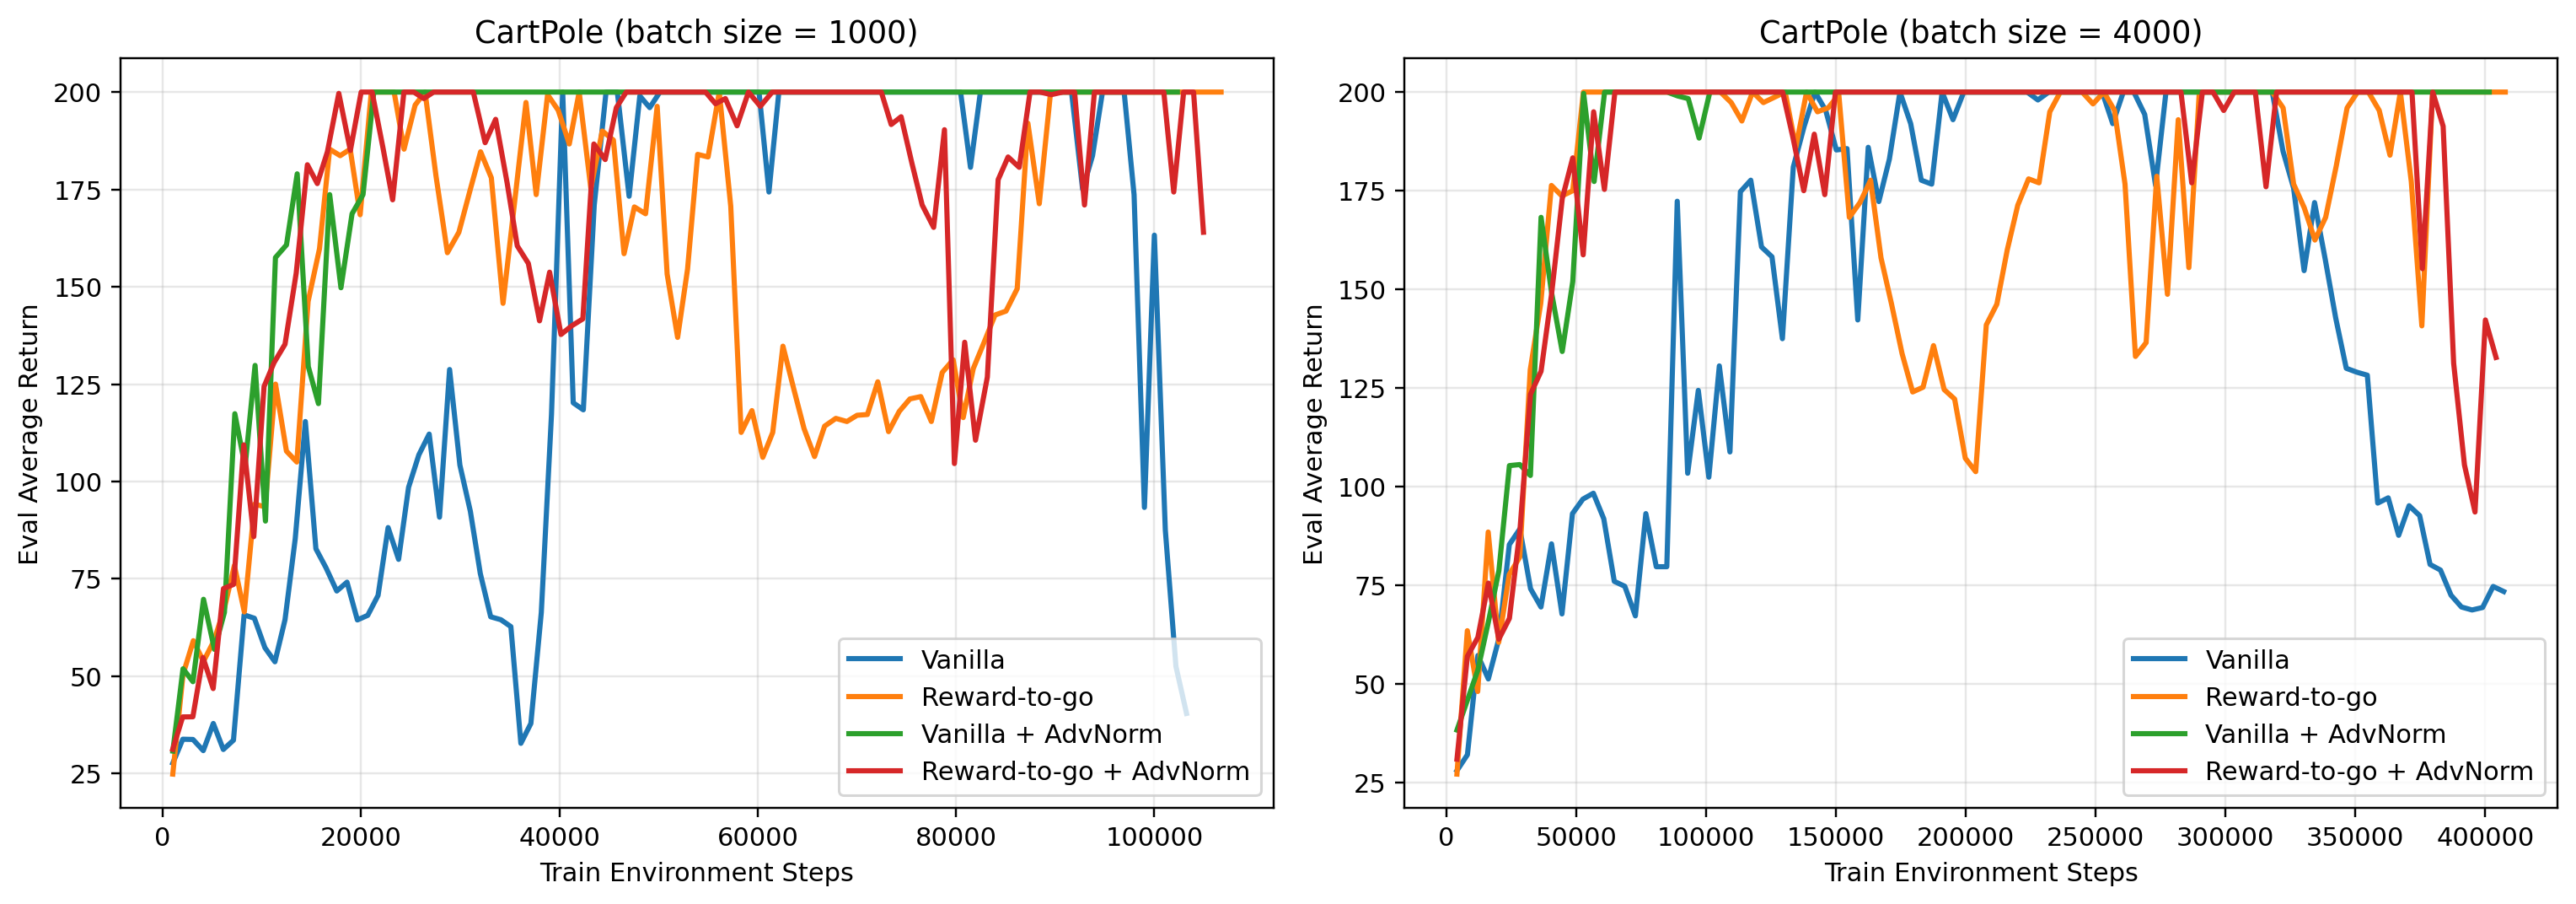
\includegraphics[width=\textwidth]{assets/exp1_cartpole_comparison.png}
    \caption{CartPole-v0 learning curves. The left panel uses batch size $1000$ and the right panel uses batch size $4000$; the x-axis is Train\_EnvstepsSoFar and the y-axis is Eval\_AverageReturn. The plot compares vanilla PG, reward-to-go, and advantage-normalized variants.}
\end{figure}

\subsubsection{Questions:}

Answer the following questions briefly:
\begin{itemize}
    \item Which value estimator has better performance without advantage normalization: the sum of trajectory rewards (REINFORCE) or the one using reward-to-go? \\
    \textbf{Answer:} Reward-to-go performed better. In both batch settings, the reward-to-go run reached the maximum score of 200 much earlier and stayed more stable, whereas vanilla REINFORCE learned more slowly and its final return remained much lower (about 40.4 for $b=1000$ and 73.4 for $b=4000$ in this run).
    \item Did advantage normalization help? \\
    \textbf{Answer:} Yes overall, but mainly for the vanilla estimator. Advantage normalization made the vanilla PG runs much more sample-efficient and both normalized vanilla runs reached 200 quickly. For reward-to-go, normalization did not clearly help in my runs, since reward-to-go already learned well and the normalized reward-to-go runs were slightly less stable near the end.
    \item Did the batch size make an impact? \\
    \textbf{Answer:} Yes, but mostly in stability rather than final solvability. Larger batches produced somewhat smoother curves, but they did not improve sample efficiency in terms of environment steps; the best small-batch runs reached 200 earlier than the best large-batch runs. In both settings, reward-to-go and vanilla with advantage normalization were enough to solve CartPole.
    \item Provide the exact command line configurations you used to run your experiments, including any parameters changed from their defaults. \\
    \textbf{Answer:}
\begin{verbatim}
python cas4160/scripts/run_hw2.py --env_name CartPole-v0 -n 100 -b 1000 --exp_name cartpole
python cas4160/scripts/run_hw2.py --env_name CartPole-v0 -n 100 -b 1000 -rtg --exp_name cartpole_rtg
python cas4160/scripts/run_hw2.py --env_name CartPole-v0 -n 100 -b 1000 -na --exp_name cartpole_na
python cas4160/scripts/run_hw2.py --env_name CartPole-v0 -n 100 -b 1000 -rtg -na --exp_name cartpole_rtg_na
python cas4160/scripts/run_hw2.py --env_name CartPole-v0 -n 100 -b 4000 --exp_name cartpole_lb
python cas4160/scripts/run_hw2.py --env_name CartPole-v0 -n 100 -b 4000 -rtg --exp_name cartpole_lb_rtg
python cas4160/scripts/run_hw2.py --env_name CartPole-v0 -n 100 -b 4000 -na --exp_name cartpole_lb_na
python cas4160/scripts/run_hw2.py --env_name CartPole-v0 -n 100 -b 4000 -rtg -na --exp_name cartpole_lb_rtg_na
\end{verbatim}
\end{itemize}

\section{Using a Neural Network Baseline}
\label{sec:nn_baseline}

\subsection{Implementation}

I implemented the value function baseline, trained it jointly with the policy, and subtracted the learned value prediction from reward-to-go to form the advantage estimate. I also added support for multiple baseline gradient steps per policy update.

\subsection{Experiments}
\textbf{Experiment 2 (HalfCheetah).} I compared policy gradient with and without the learned baseline, and then ran one additional ablation with reduced baseline updates using \texttt{-blr 0.005 -bgs 2}.

\subsection*{Deliverables:}
\begin{itemize}
    \item Plot a learning curve for the baseline loss.
    \item Plot a learning curve for the eval return.
    \item Run another experiment with a decreased number of baseline gradient steps (\texttt{-bgs}) and/or baseline learning rate (\texttt{-blr}). How does this affect (a) the baseline learning curve and (b) the performance of the policy?
\end{itemize}

\subsection*{What to Expect:}
\begin{itemize}
  \item You should expect to achieve an average return over $300$ for the baseline version.
\end{itemize}

\subsection{Neural Network Baseline Result}

\subsubsection{Plot (Baseline Loss, Eval Average Return):}

\begin{figure}[H]
    \centering
    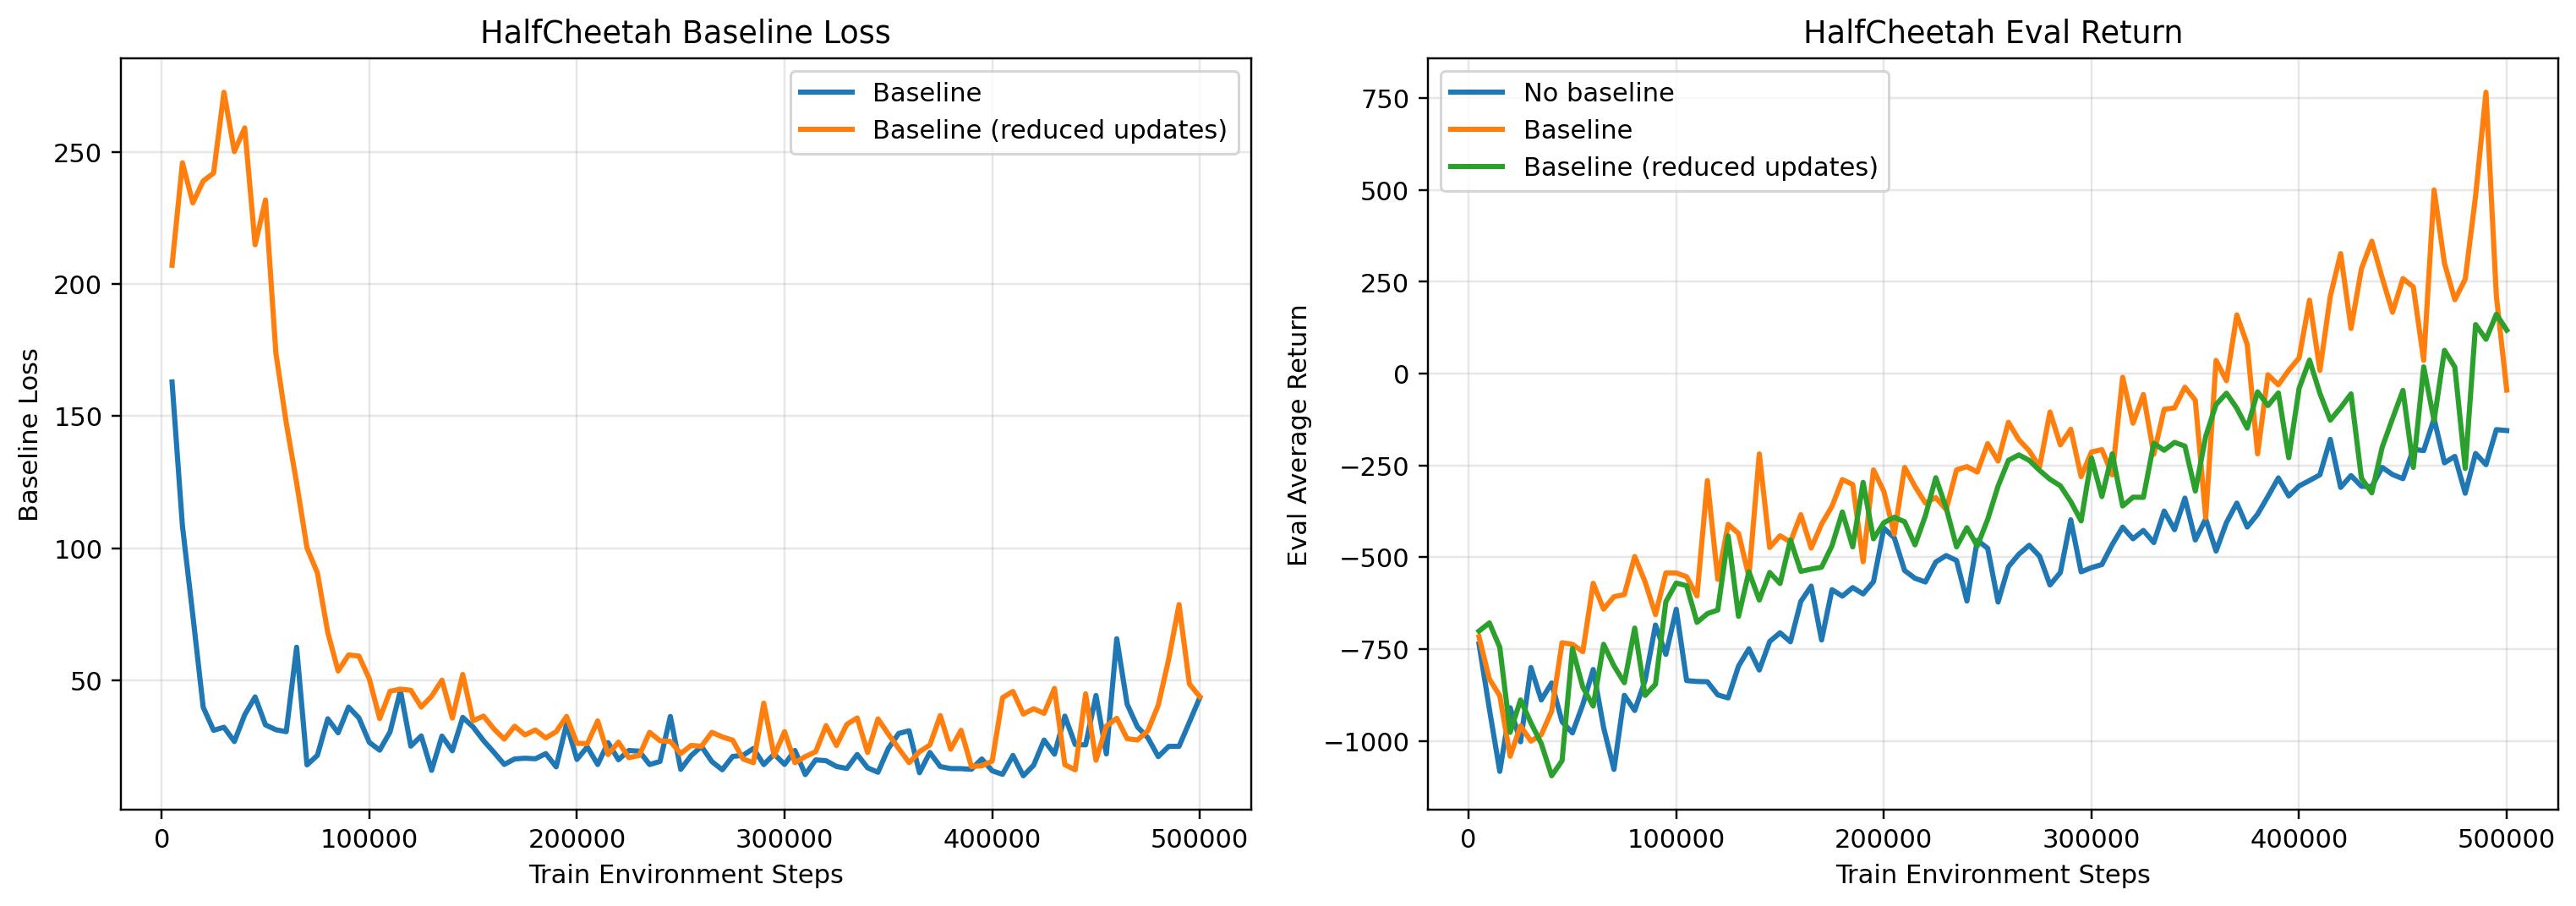
\includegraphics[width=\textwidth]{assets/exp2_cheetah_baseline.png}
    \caption{HalfCheetah-v4 results. The left panel shows baseline loss, and the right panel shows Eval\_AverageReturn. We compare no baseline, the default baseline setting, and a reduced baseline-update ablation (\texttt{-blr 0.005, -bgs 2}) to show how critic update strength affects policy learning.}
\end{figure}

\subsubsection{Questions:}

Answer the following questions briefly:
\begin{itemize}
    \item Run another experiment with a decreased number of baseline gradient steps (\texttt{-bgs}) and/or baseline learning rate (\texttt{-blr}). How does this affect (a) the baseline learning curve and (b) the performance of the policy? \\
    \textbf{Answer:} I ran:
\begin{verbatim}
python cas4160/scripts/run_hw2.py --env_name HalfCheetah-v4 \
    -n 100 -b 5000 -rtg --discount 0.95 -lr 0.01 \
    --use_baseline -blr 0.005 -bgs 2 --exp_name cheetah_baseline_lowb
\end{verbatim}
Compared with the default baseline run (\texttt{-blr 0.01 -bgs 5}), the reduced-update setting learned a weaker critic: the baseline loss started higher (207.1 vs.\ 162.9), reached its minimum later, and stayed slightly worse at its best point (16.05 vs.\ 13.79). The policy still improved substantially over the no-baseline run and even finished with a positive return (118.35), but its peak return was much lower than the default baseline run (161.48 vs.\ 766.10), so reducing critic updates hurt overall policy quality and sample efficiency.
\end{itemize}

\section{Generalized Advantage Estimator}
\label{sec:gae}

\subsection{Implementation}
I implemented GAE-$\lambda$ in \texttt{PGAgent.\_estimate\_advantage()} using the recursive form with temporal-difference residuals.

\subsection{Experiments}
\textbf{Experiment 3 (HumanoidStandup-v5).} I tested $\lambda \in \{0, 0.95, 1\}$ using the required hyperparameters.

\subsection*{Deliverables:}
\begin{itemize}
    \item Provide a single plot with the learning curves for the \texttt{HumanoidStandup-v5} experiments that you tried.
    \item Describe in words how $\lambda$ affected task performance and training efficiency.
    \item Consider the parameter $\lambda$. What does $\lambda=0$ correspond to? What about $\lambda=1$?
\end{itemize}

\subsection*{What to Expect:}
\begin{itemize}
  \item The run with the best performance should achieve an average score close to $1.15e4$.
\end{itemize}

\subsection{GAE Result}
\subsubsection{Plot (Eval Average Return with different $\lambda$):}

\begin{figure}[H]
    \centering
    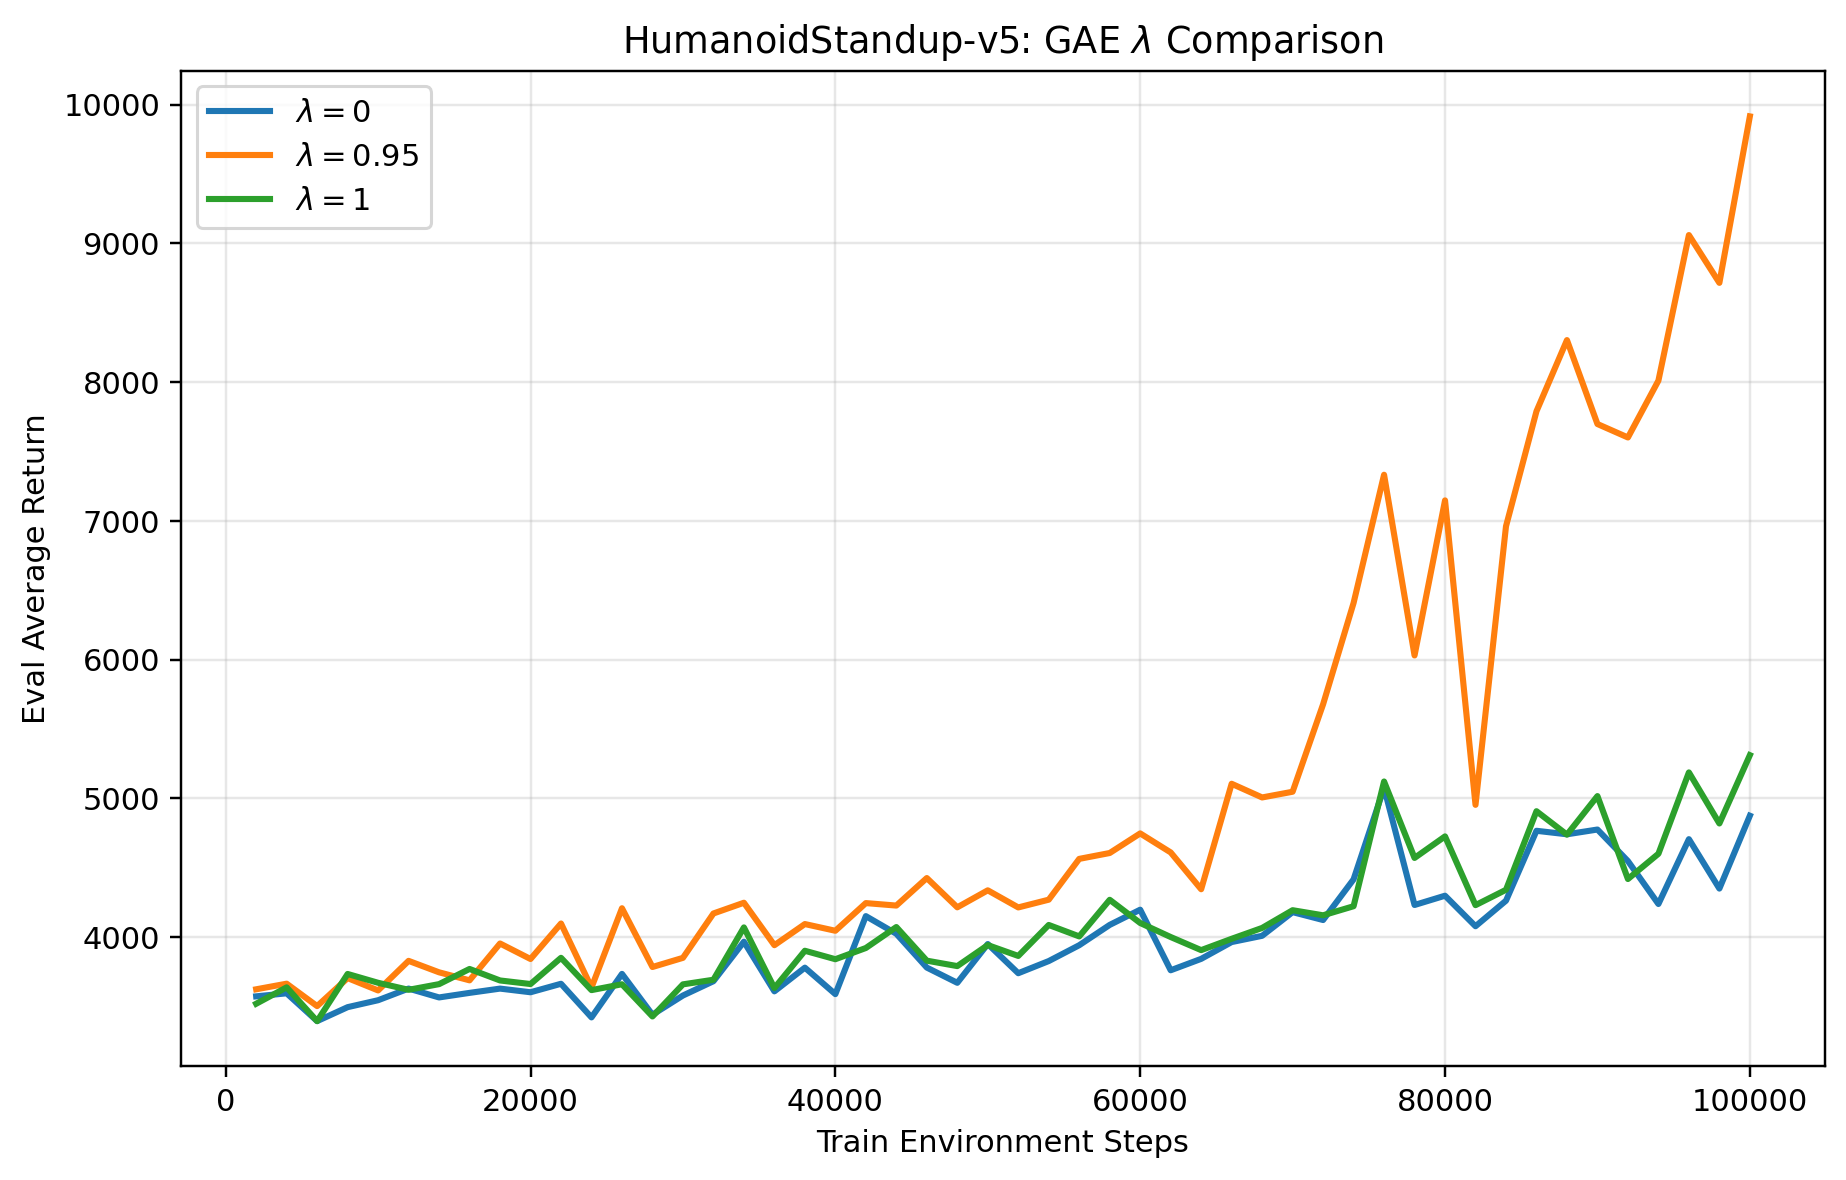
\includegraphics[width=0.85\textwidth]{assets/exp3_humanoid_gae.png}
    \caption{HumanoidStandup-v5 Eval\_AverageReturn for different GAE values ($\lambda \in \{0, 0.95, 1\}$). The intermediate setting $\lambda=0.95$ shows the best overall learning trend, indicating a better bias-variance tradeoff than either extreme.}
\end{figure}

\subsubsection{Questions:}

Answer the following questions briefly:
\begin{itemize}
    \item Describe in words how $\lambda$ affected task performance. \\
    \textbf{Answer:} $\lambda$ had a large effect. The intermediate setting $\lambda=0.95$ worked best by a wide margin, reaching about 9916 final eval return, while $\lambda=0$ and $\lambda=1$ only reached about 4874 and 5311 respectively. In this task, an intermediate bias-variance tradeoff was clearly better than either extreme.
    \item Consider the parameter $\lambda$. What does $\lambda=0$ correspond to? What about $\lambda=1$ ? Relate this to the task performance in \texttt{HumanoidStandup-v5} in one or two sentences. \\
    \textbf{Answer:} $\lambda=0$ corresponds to the one-step TD advantage estimate $\delta_t$, which has lower variance but higher bias. $\lambda=1$ corresponds to the Monte Carlo-style advantage estimate, which has lower bias but higher variance. On \texttt{HumanoidStandup-v5}, neither extreme was best; $\lambda=0.95$ gave the best balance and therefore the best learning curve.
\end{itemize}

\section{Proximal Policy Optimization}
\label{sec:ppo}

Finally, I implemented PPO-Clip and used generalized advantage estimates to form the surrogate objective. PPO constrains policy changes by clipping the probability ratio, which makes it possible to reuse on-policy data for multiple minibatch updates without destabilizing training.

\subsection{Implementation}
I implemented the clipped PPO objective in \texttt{MLPPolicyPG.ppo\_update()} and integrated PPO minibatch updates into \texttt{PGAgent.update()}.

\subsection{Experiments}
\textbf{Experiment 4 (Reacher-v4).} I compared the baseline policy gradient agent and PPO using the required settings.

\subsection*{Deliverables:}
\begin{itemize}
    \item Provide a single plot with the learning curves for the Reacher-v4 experiments that you tried.
    \item Compare the performances of the final agent with and without using PPO.
    \item If we do not use surrogate objective and do multiple batch updates, what would happen? Justify the result.
\end{itemize}

\subsection*{What to Expect:}
\begin{itemize}
  \item The run with PPO should achieve an average score close to $-10$ if correctly implemented (at least $-15$).
\end{itemize}

\subsection{PPO Result}
\subsubsection{Plot (Eval Average Return for PPO and the baseline):}

\begin{figure}[H]
    \centering
    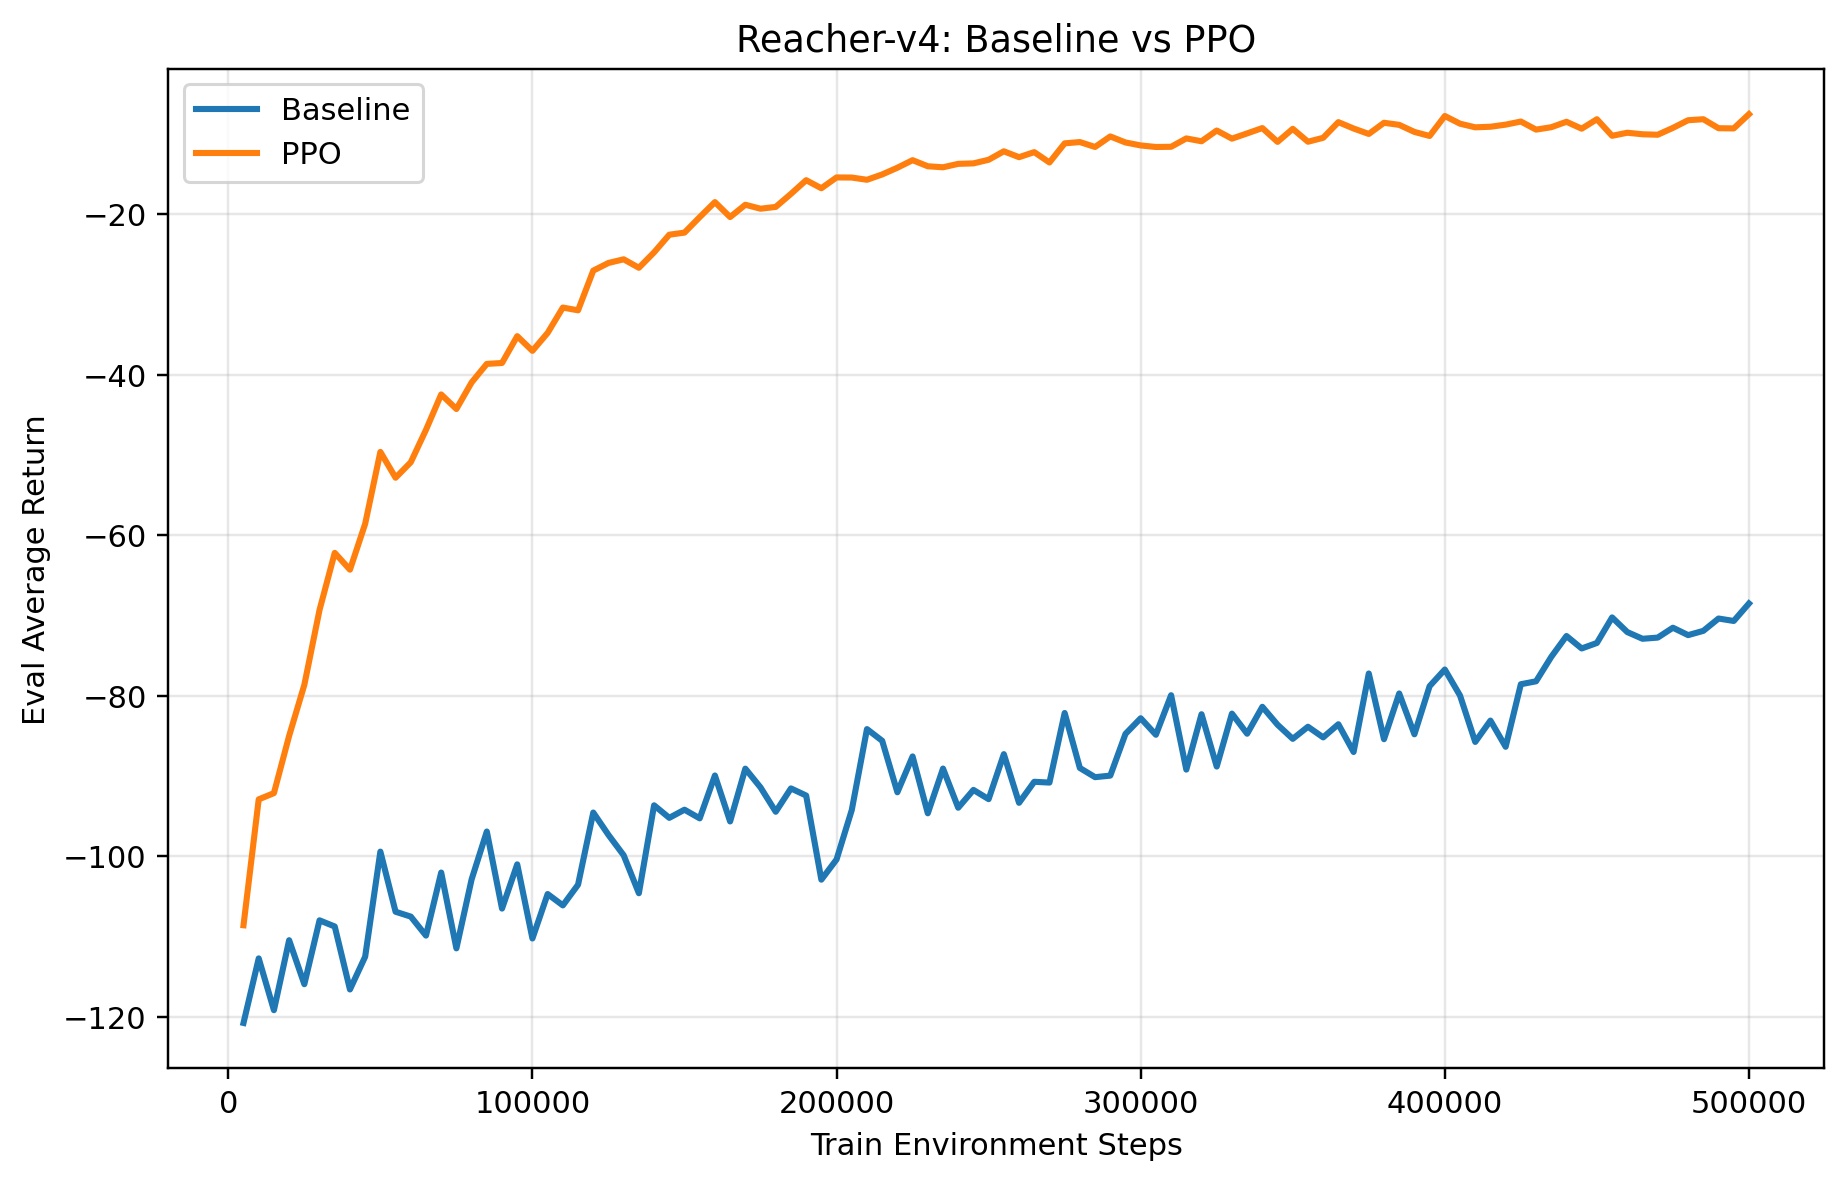
\includegraphics[width=0.85\textwidth]{assets/exp4_reacher_ppo.png}
    \caption{Reacher-v4 comparison between baseline PG (with GAE) and PPO. Under the same base hyperparameters, PPO improves more steadily and reaches a substantially better final Eval\_AverageReturn (about $-7.53$) than the baseline (about $-68.50$).}
\end{figure}

\subsubsection{Questions:}

Answer the following questions briefly:
\begin{itemize}
    \item If we do not use surrogate objective and do multiple batch updates, what would happen? Justify the result. \\
    \textbf{Answer:} Training would usually become unstable and can even collapse. Without the clipped surrogate objective, repeatedly updating on the same on-policy batch keeps pushing the policy using data collected from an increasingly outdated policy, so the effective policy ratio can drift too far from $1$. That breaks the trust-region-like effect of PPO, causes overly large policy updates, and typically hurts performance instead of improving it.
\end{itemize}

\section{Submission}

Please include the code, tensorboard logs data, and the \textbf{report}. Zip it to \texttt{hw2\_[YourStudentID].zip}. The structure of the submission file should be:

\begin{forest}
  for tree={
    font=\ttfamily,
    grow'=0,
    child anchor=west,
    parent anchor=south,
    anchor=west,
    calign=first,
    edge path={
      \noexpand\path [draw, \forestoption{edge}]
      (!u.south west) +(7.5pt,0) |- node[fill,inner sep=1.25pt] {} (.child anchor)\forestoption{edge label};
    },
    before typesetting nodes={
      if n=1
        {insert before={[,phantom]}}
        {}
    },
    fit=band,
    before computing xy={l=15pt},
  }
  [{hw2\_2021147505.zip}
    [{hw2\_2021147505.pdf}]
    [cas4160/
      [{...codes}]
    ]
    [...]
  ]
\end{forest}

\textbf{Note: Do NOT include the videos (.mp4 files or tensorboard logs) in your submission. Your submission file size should be less than 50MB.}

\end{document}
